% !TeX encoding = UTF-8
% !TeX TS-program = pdflatex
% !TeX spellcheck = de_DE

\def\version{\today L. Schink}
% Verlauf
% v 1.1 20.2.20202 S. Schramm - Initiale Version
% v 1.2 20.2.20202 A. Dürrbaum - Anpassungen Ttielseite / Indices

% Dokumenteneinstellung
\documentclass[a4paper,11pt,cleardoubleempty]{scrbook}

%% Einstellungsdatei
% !TeX spellcheck = de_DE

% Do's & Dont's in LaTeX
%\RequirePackage[l2tabu,orthodox]{nag}

% Deutsch und UTF-8 Encoding
\usepackage[english,ngerman]{babel}
\selectlanguage{ngerman}

\usepackage[utf8]{inputenc}
\usepackage[T1]{fontenc}
\usepackage{lmodern}

% Seiteneinstellungen
\usepackage{geometry}
\geometry{left=35mm,right=35mm, bindingoffset=0mm, top=30mm,bottom=30mm}

% Abstand im Text
\usepackage{xspace}
\usepackage{setspace}

% Kapitelüberschrift: große Nummer -> Titel
\renewcommand*{\chapterformat}{\mbox{\chapappifchapterprefix{\nobreakspace}\scalebox{3}{\thechapter}\enskip}}

% Linie unter \chapter
\makeatletter
\renewcommand{\chapterlinesformat}[3]{%
  \parbox[t]{\linewidth}{%
    \raggedchapter\@hangfrom{#2}{#3}\par%
    \vspace*{-.75\ht\strutbox}\rule{\linewidth}{.8pt}%
  }%
}
\makeatother

% pdf Pakete
\usepackage[pdfusetitle=true,colorlinks=true,linkcolor=blue,urlcolor=blue,citecolor=blue,bookmarks=true,bookmarksopenlevel=2]{hyperref}

% Pakete für Grafiken
\usepackage{graphicx}
\usepackage{color}
\usepackage{xcolor}
\usepackage{tikz}
\usepackage{pgfplots}
\pgfplotsset{compat=1.5}
\usepackage{caption}
\captionsetup{labelfont=bf, textfont=small} 
\usepackage{subcaption}

% Tabellentools
\usepackage{supertabular}
\usepackage{multirow}
\usepackage{multicol}

% Mathematik
\usepackage[fleqn]{amsmath}
\usepackage{amssymb,amsthm,textcomp}
\usepackage{upgreek}

% Zahlenformate
\usepackage{siunitx}
\sisetup{range-phrase=\ \textrm{bis}\ }
\sisetup{locale=DE}

% Auflistungen
\usepackage{enumerate}
\usepackage{enumitem}

% Symbolverzeichnis
\usepackage[nomentbl]{Einstellungen/nomencl-table}

% Glossar
%\usepackage[nonumberlist,toc,nopostdot,style=alttree,xindy]{glossaries}
\usepackage{glossaries}

% Index
\usepackage{makeidx}

% Listings
\usepackage{listings}

% Eigene Tabellenspalten
\usepackage{tabularx}
\usepackage{dcolumn}

%%%%%%%%%%%%%%%%%%%%%%%%%%%%%%%%%%%%%%%%%%%%%%%%%%%%%%%%%%%%%%%%%%%%%%%%%%%%%%
% HIER EIGENE PAKETE HINZUFÜGEN
%
%
%
%
%%%%%%%%%%%%%%%%%%%%%%%%%%%%%%%%%%%%%%%%%%%%%%%%%%%%%%%%%%%%%%%%%%%%%%%%%%%%%%
% Vor dem Laden von weiteren Paketen in das Latex-Sündenregister von Marc Ensenbach schauen!
%%%%%%%%%%%%%%%%%%%%%%%%%%%%%%%%%%%%%%%%%%%%%%%%%%%%%%%%%%%%%%%%%%%%%%%%%%%%%%

%%%%% Sonstiges
\usepackage{grffile}

% Es können todo-Notes eingefügt werden
\usepackage{todonotes}

% Definition der Kopf und Fußzeilen
\usepackage{fancyhdr,lastpage}
\fancypagestyle{fancy2}{%
	\fancyhf{}
	\fancyhead[L]{}
	\fancyhead[C]{}
	\fancyhead[R]{}
	\fancyfoot[OL]{}
	\fancyfoot[EL]{\thepage}
	\fancyfoot[C]{ }
	\fancyfoot[OR]{\thepage}
	\fancyfoot[ER]{}
	\renewcommand{\headrulewidth}{1pt}
	\renewcommand{\footrulewidth}{1pt}
}
\fancypagestyle{plain}{%
	\fancyhf{}%
	\renewcommand{\headrulewidth}{0pt}%
	\renewcommand{\footrulewidth}{0pt}
	\fancyfoot[OR]{\thepage}
}
\renewcommand{\headrulewidth}{0pt}
\renewcommand{\footrulewidth}{0pt}
\usepackage{emptypage}

% \matr{A} ergibt "fettes A" wie es bei Matrizen aussehen soll
\newcommand{\matr}[1]{\mathbf{#1}}

% Definition der Uni Kassel Farbpalette
\definecolor{UKDunkelGrau}{RGB}{87,87,87}
\definecolor{UKMittelGrau}{RGB}{157,157,157}
\definecolor{UKHellGrau}{RGB}{218,218,218}
\definecolor{UKDunkelPink}{RGB}{154,12,70}
\definecolor{UKMittelPink}{RGB}{199,16,92}
\definecolor{UKHellPink}{RGB}{243,216,221}
\definecolor{UKGruen}{RGB}{21,56,36}
\definecolor{UKBlau}{RGB}{80,149,200}
\definecolor{UKGelb}{RGB}{196,210,15}
\definecolor{UKTuerkis}{RGB}{74,172,150}
\definecolor{UKGold}{RGB}{234,195,114}

%%%%%%%%%%%%%%%%%%%%%%%%%%%%%%

\renewcommand{\familydefault}{\rmdefault}
\renewcommand*\rmdefault{ppl}

\setlength{\parindent}{0pt}
\setlength{\parskip}{6pt}

\makeatletter
% !TeX spellcheck = de_DE
\renewcommand{\maketitle}{\fontfamily{cmss}\selectfont
  \begin{center}
	\vspace*{-0.5cm}
	
\includegraphics[width=75mm]{Bilder/UniKS-Logo}\\

	\vspace{1.5cm}
	\centering
        \ifthenelse{\equal{\Typ}{MSc}}{
	% Masterarbeit
	\textbf{\Large Masterarbeit}\\[1ex]
        }{\ifthenelse{\equal{\Typ}{BSc}}{
	% Bachelorarbeit
	\textbf{\Large Bachelorarbeit}\\[1ex]
        }{
        %  Restliche Arbeiten:
	\textbf{\Large \Typ}\\[4ex]
        }}
	\textsf{\Huge \@title}\\[4ex]
%
	{\Large \@author}\\[4ex]
%
        \ifthenelse{\isundefined{\Titelgrafik}}{}{
  	  \vfill
          \includegraphics[height=8cm]{\Titelgrafik}
  	  \vfill
        }
	\vfill
        \ifthenelse{\equal{\Typ}{Technischer Bericht}}{
        Bericht-Nr. \MRTnr\\  
        }{ 
        \begin{center}
          %\fbox{\parbox{14cm}{
          \renewcommand{\arraystretch}{1.2}
		\begin{tabularx}{\columnwidth}{p{0.5\textwidth}>{\raggedleft\arraybackslash}p{0.5\textwidth}}
			Matrikelnummer: & \MatNr\\
                        \ifthenelse{\equal{\Typ}{MSc}\or\equal{\Typ}{BSc}}{
			Erstgutachter: & \Erstgutachter\\
			Zweitgutachter: & \Zweitgutachter\\}{
			Gutachter: & \Erstgutachter\\}
                        \ifthenelse{\isundefined{\Betreuer}}{}{
			Betreuer: & \Betreuer\\}
			Tag der Abgabe: & \@date\\
                        \ifthenelse{\isundefined{\MRTnr}}{}{MRT-Nr.:& \MRTnr\\}
                      \end{tabularx}%
            %          }}
                    \end{center}
        }
	\vfill
	
\includegraphics[height=12mm]{Bilder/MRT-Logo} \hfill 
\includegraphics[height=12mm]{Bilder/ISAC-Logo}
\end{center}
}


%%% Local Variables:
%%% mode: latex
%%% TeX-master: "../MRT-Bericht-2020"
%%% End:

\makeatother

\newcounter{SeitenzahlSpeicher}

%%% Local Variables:
%%% mode: latex
%%% TeX-master: "../MRT-Bericht-2020"
%%% End:


%% Alternative zu Schriftart Calibri
\usepackage[sfdefault,lf]{carlito}


%% Benötigte Daten!
\title{\fontsize{16}{14}\selectfont Implementierung einer robotergestützten Lagerverwaltung in Python\\
{\fontsize{10}{10}\selectfont Mit kameragestützen Validierungsprozessen in der Industrie 4.0-Plattform Modellfabrik $\mu$Plant}}
\date{\today}
\author{Lennart Schink}
\def\MatNr{33237484}
 
%% Wenn \geburtsort auskommentiert -> Ausgabe von
%%  Geburtsag und Geburtsort auf Deckblatt
\def\Geburtsort{Bad Bergzabern}\def\Geburtstag{31.12.1990}

%% Art des Berichtes (eines auskommentieren)
%\def\Typ{MSc}
%\def\Typ{Seminararbeit}
\def\Typ{BSc}
%\def\Typ{Seminararbeit}
%\def\Typ{Technischer Bericht}

%% MRT-Nummer, wenn schon bekannt
\def\MRTnr{N.N}

%% Auskommentieren, wenn eine Grafig auf dem Titelblatt erscheinen sollen
% maximale Höhe: 5cm, max. Breite 15 cm
%\def\Titelgrafik{Bilder/Wissenschaft.jpg}

%% Gutachter
\def\Erstgutachter{Univ.-Prof.~Dr.-Ing. Andreas Kroll}
\def\Zweitgutachter{Dr.-Ing. Robert Schmoll } % nur bei MSc oder BSc

%% Auskommentieren, wenn der/die Betreuer auf dem Titelblatt erscheinen sollen
\def\Betreuer{Dip.-Ing. Axel Dürrbaum} % Mehrer Betreuer möglich

%% PDF mit Aufgabenstellung
\def\Aufgabenstellung{Bilder/Aufgabenstellung.pdf}

%% MRT-Informationen im PDF
\pdfinfo{
   /Author \@author
   /Title \@title
   /CreationDate \@date
   /Subject \Typ
   /Keywords (MRT;LaTeX)
}


% --------------------------------------------------------------------
% Benutzerdefinierte Makros
% --------------------------------------------------------------------

% Schreibweise für Vektoren
\def\Vektor#1{\ensuremath{\mathbf{#1}}}

% Transponieren einesVektors/einer Matrix
\def\Trans#1{\ensuremath{#1^{\mathrm{T}}}}

% Variable/Zahlenwert mit Einheit
\def\Einheit#1#2{\ensuremath{#1 \text{ in } \mathrm{#2}}}

% --------------------------------------------------------------------
% Abkürzungsverzeichnis
\makeglossary
\newcommand*{\Glossar}[3]{#3 (\gls{#1})\newglossaryentry{#1}{name=#2,
    description={#3}}}

% Symbolverzeichnis
\makenomenclature
\renewcommand{\nomname}{Symbolverzeichnis}
\newcommand*{\Symbol}[2]{#1\nomenclature{#1}{#2}{}{}}
\newcommand*{\SymbolT}[2]{#2 #1\nomenclature{#1}{#2}{}{}}
\newcommand*{\SymbolE}[3]{#2 #1\nomenclature{#1}{#2}{#3}{}}
\newcommand*{\SymbolB}[4]{#2 #1\nomenclature{#1}{#2}{#3}{#4}}

% Index
\makeindex
\newcommand*{\Index}[1]{#1\index{#1}}

% --------------------------------------------------------------------
  
% Beginn des Dokuments
\begin{document}
\pagenumbering{Roman}

% Bei Problemen mit überhängenden Absätzen kann Sloppy zur Aufweichung
% der Satzparameter genutzt werden. Dies wird offiziell nicht
% empfohlen, kann aber u. U. zu guten Ergebnissen führen.
%\sloppy

% --------------------------------------------------------------------------
% Titelseite (IMMER)
% --------------------------------------------------------------------------
\fancyhf{}
\pagestyle{empty}
\maketitle 
\cleardoublepage

% --------------------------------------------------------------------------
% Aufgabenstellung (IMMER) 
% PDF-Aufgabenstellung von Betreuer geben lassen und hier einfügen
% --------------------------------------------------------------------------
\ifthenelse{\equal{\Typ}{MSc}\or\equal{\Typ}{BSc}}{
\begin{figure}[!htbp]\centering
\fbox{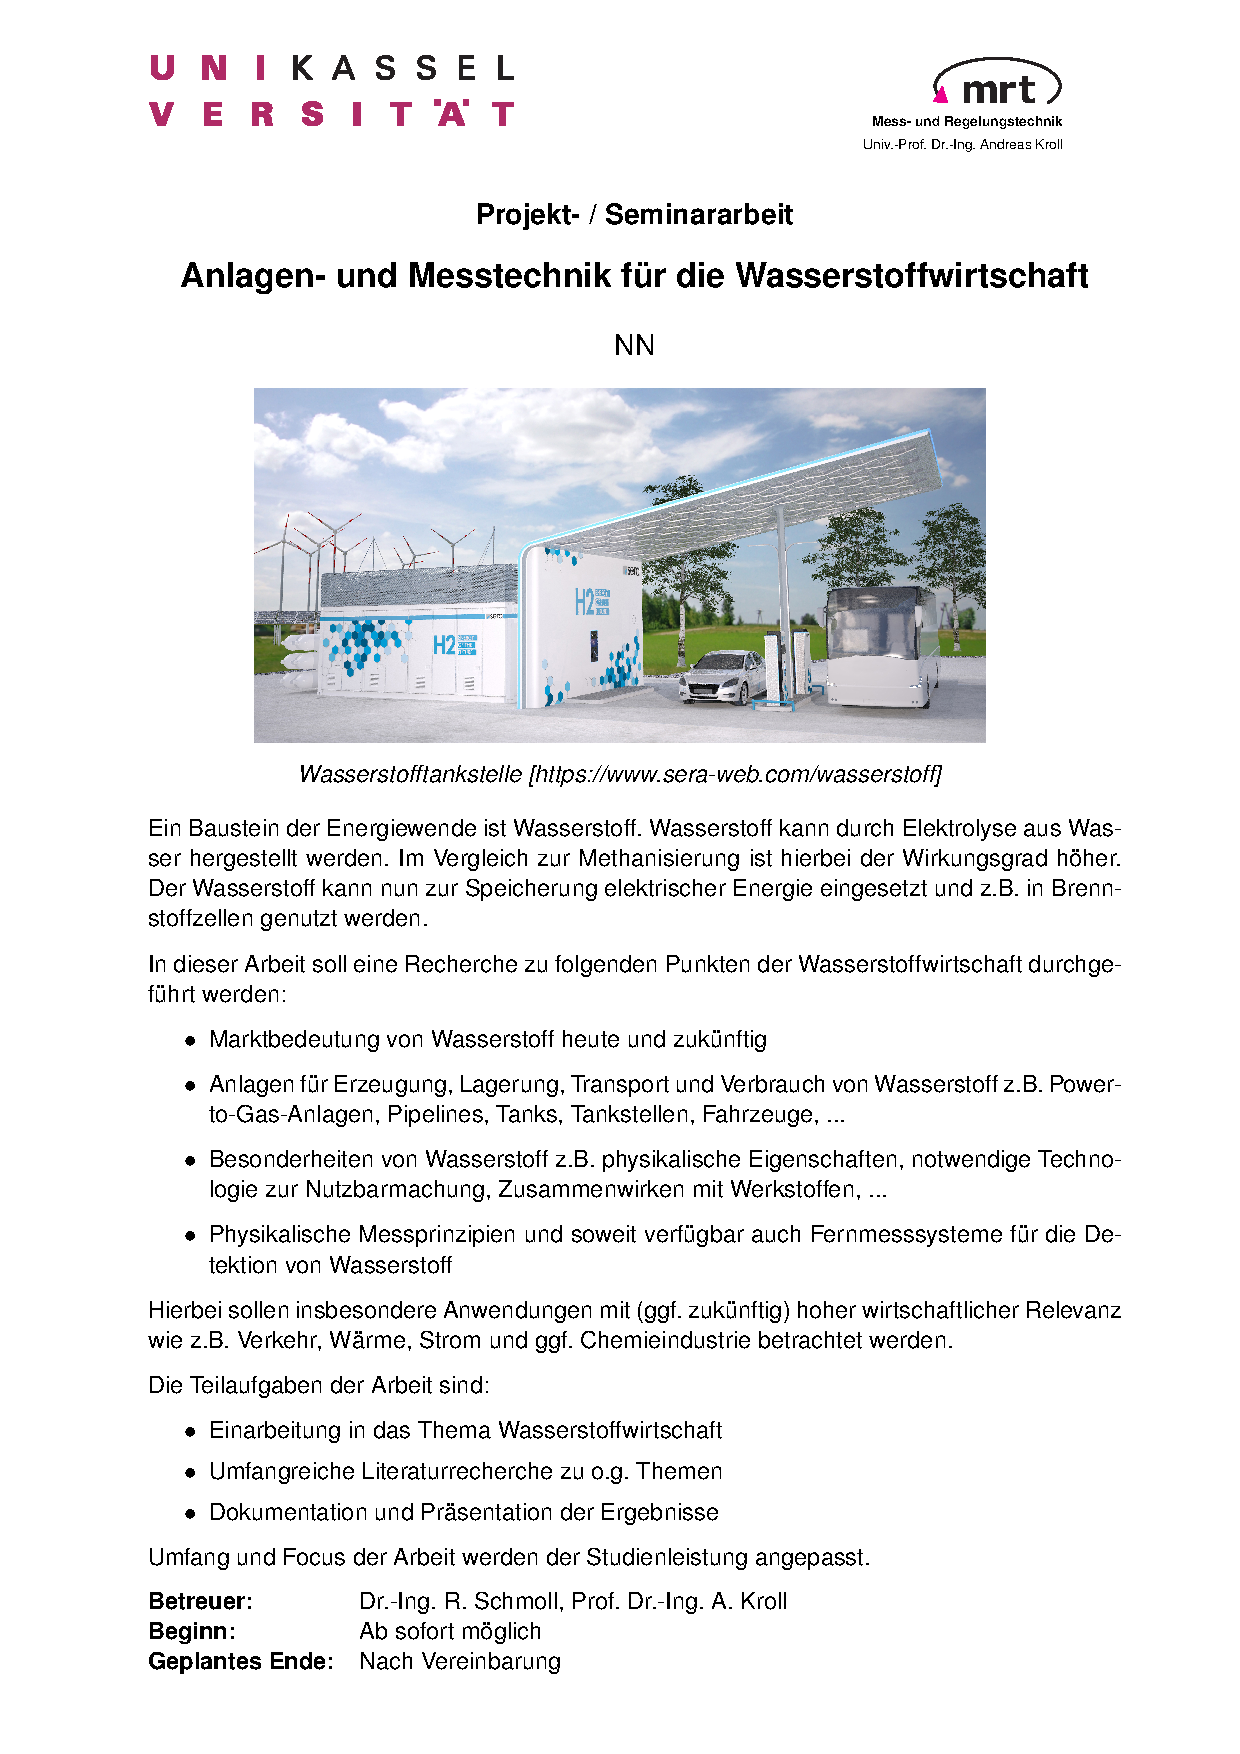
\includegraphics[width=1.0\textwidth,page=1]{\Aufgabenstellung}}
\end{figure}

\begin{figure}[!htbp]
\centering
\fbox{\includegraphics[width=1.0\textwidth,page=2]{\Aufgabenstellung}}
\end{figure}
\cleardoublepage
}{}

% --------------------------------------------------------------------------
% Versicherung (BEI BA UND MA)
% --------------------------------------------------------------------------
\ifthenelse{\equal{\Typ}{MSc}\or\equal{\Typ}{BSc}}{
% !TeX encoding = UTF-8
% !TeX TS-program = pdflatex
% !TeX spellcheck = de_DE

\chapter*{Versicherung}

Hiermit versichere ich, dass ich die vorliegende Arbeit selbstständig
verfasst und keine anderen als die angegebenen Quellen und Hilfsmittel
verwendet habe.

\vspace*{5ex}
\rule{12cm}{0.5pt}\newline
Ort, Datum, Unterschrift


%%% Local Variables:
%%% mode: latex
%%% TeX-master: "../MRT-Bericht2020"
%%% End:

\cleardoublepage
}{}

% --------------------------------------------------------------------------
% Zusammenfassung (BEI BA UND MA)
% --------------------------------------------------------------------------
\ifthenelse{\equal{\Typ}{MSc}\or\equal{\Typ}{BSc}}{
% !TeX spellcheck = de_DE
\chapter*{Kurzfassung}

Diese Bachelorarbeit widmet sich der Untersuchung des Einsatzes optischer Marker zur Verbesserung von Inventurprozessen in automatischen Lagerzellen. 
Die Arbeit stützt sich auf Erkenntnisse aus den Arbeiten von \cite[Hübler (2019)]{Hübler2019} und \cite[Kistner (2017)]{LarsKistner2017}  auf
und nutzt zwei Kameras zur Markererkennung: Eine Übersichtskamera in der oberen Ecke der Lagerzelle und eine Kamera, die am Greifer angebracht ist.

Die Implementierung der Inventurprozesse erfolgt in der Warehouse Management Software, wobei Python 3.11 im Backend und das Qt Framework mit PySide6 Bindings 
im Frontend verwendet werden. 
Die Bildverarbeitung und Markererkennung erfolgt mithilfe der Open-Source-Bibliothek OpenCV, und die perspektivische 
Entzerrung wird mit scikit-image durchgeführt.

Im Vorfeld dieser Arbeit wurden umfangreiche Vorarbeiten im Rahmen meiner \cite[Semesterarbeit]{Semesterarbeit} geleistet, 
darunter die Erarbeitung einer Softwarearchitektur für die bestehende Lagerverwaltungssoftware Lagerverwaltung 3.0 (Rodriguez, 2019) 
sowie Überlegungen zur Auswahl der Kameras. Anlass zur Neuimplementierung der Lagerverwaltungssoftware ist der Wunsch einer 
eiheitlichen Programmiersprache in der Modellfabrik $\mu$Plant und der Wechsel des Betriebssystems von Windows 7 auf Windows 10.
Die ursprüngliche Implementierung in C$\#$ funktioniert nicht mehr fehlerfrei unter Windows 10.
Außerdem baut die alte Implementierung auf dem Protokoll Modbus auf, das in der $\mu$Plant durch den Industriestandard OPC UA ersetzt wird.

Die Arbeit beinhaltet viele Aspekte der modernen Softwareentwicklung, einschließlich der Implementierung von Plug-Ins, 
Integration von Legacy-Schnittstellen, portierung der M2M-Kommunikation von Modbus nach OPC UA und eine Forschungskomponente z
ur arUco Marker-Erkennung. 

Abschließend werden eigene Überlegungen zur grundsätzlichen Erkennung der Behälter präsentiert, 
die als Anregung für zukünftige Forschungsarbeiten dienen sollen.

\ifthenelse{\equal{\Typ}{MSc}}{
\vfill
\section*{Summary}
\begin{otherlanguage}{english}
Awaken the reader's interest here!

Why should he read this - exactly this - work?
\end{otherlanguage}

\selectlanguage{ngerman}
}{}

%%% Local Variables:
%%% mode: latex
%%% TeX-master: "../MRT-Bericht-2020"
%%% End:

\cleardoublepage
}{}

% --------------------------------------------------------------------------
% Summary (BEI MA)
% --------------------------------------------------------------------------
%\ifthenelse{\equal{\Typ}{MSc}}{
%\include{Kapitel/Summary}
%\cleardoublepage
%}{}

% --------------------------------------------------------------------------
% Inhaltsverzeichnis (IMMER)
% --------------------------------------------------------------------------
\tableofcontents
\cleardoublepage

% --------------------------------------------------------------------------
% Liste der Tabellen und Bilder und Listings
% --------------------------------------------------------------------------
\listoftables      % optional
\listoffigures     % optional
\lstlistoflistings % optional
\cleardoublepage

% --------------------------------------------------------------------------
% Abkürzungsverzeichnis (IMMER)
% --------------------------------------------------------------------------
% !TeX spellcheck = de_DE
\chapter*{Abkürzungsverzeichnis}
\addcontentsline{toc}{chapter}{Abkürzungsverzeichnis}

\begin{center}
	
	\renewcommand{\arraystretch}{1.1}
	\tablefirsthead{\hline \textbf{Abkürzung} & \textbf{Bedeutung} \\ \hline}
	\tablehead{\hline \textbf{Abkürzung} & \textbf{Bedeutung} \\ \hline}
	
	\begin{supertabular}{p{2.1cm}p{10.9cm}}
		GUI				& \textbf{G}raphical \textbf{U}ser \textbf{I}nterface \\
		UML				& \textbf{U}nified \textbf{M}odeling \textbf{L}anguage \\
		MES				& \textbf{M}anufacturing \textbf{E}xecuting \textbf{S}ystem\\
		C\#				& An object oriented, component oriented programming language\\
		C++				& A high level, general purpose programming language\\
		QML				& \textbf{Q}t-Project's Interface \textbf{M}arkup \textbf{L}anguage\\
		LZ				& \textbf{L}ager\textbf{zelle} der $\mu$Plant\\
		FZ				& \textbf{F}ertigungs\textbf{zelle} der $\mu$Plant \\
		AuE				& \textbf{A}bfüll- \textbf{u}nd \textbf{E}ntleer - Station der $\mu$Plant \\
		RFID			& \textbf{R}adio \textbf{F}requency \textbf{ID}entification\\
		TCP/IP			& \textbf{T}ransmission \textbf{C}ontrol \textbf{P}rotocoll / \textbf{I}nternet \textbf{P}rotocoll\\
		MVC				& \textbf{M}odel - \textbf{V}iew - \textbf{C}ontroller, Ein Design-Konzept für Software\\
		URI				& \textbf{U}niform \textbf{R}essource \textbf{I}dentifier, Im Qt Framework kann dies eine beliebige
						  Ressource sein. Z.B. eine URL, ein Bild oder ein Programmteil. \\
		QML Type		& Ein QML Basiselement. Enthält alle für die Visualisierung nötigen Attribute. Eine Liste
						  aller QML Types findet sich hier \cite{qmlTypeList}\\
		RAPID			& Eine speziell für die Robotersteuerung entwickelte Programmiersprache\\
		RST				& \textbf{R}e\textbf{s}tructured \textbf{T}ext Eine einfache markup language die in Sphinx benutzt wird\\
	\end{supertabular}

\end{center}
\addcontentsline{toc}{chapter}{Abkürzungsverzeichnis}
\printglossary[title={Abkürzungsverzeichnis},toctitle={Abkürzungsverzeichnis}]
\cleardoublepage

% --------------------------------------------------------------------------
% Symbolverzeichnis (IMMER)
% --------------------------------------------------------------------------
%% !TeX spellcheck = de_DE
\chapter*{Symbolverzeichnis}
\addcontentsline{toc}{chapter}{Symbolverzeichnis}

\begin{center}
	
	\renewcommand{\arraystretch}{1.1}
	\tablefirsthead{\hline \textbf{Symbol} & \textbf{Beschreibung} & \textbf{Einheit} \\ \hline}
	\tablehead{\hline \textbf{Symbol} & \textbf{Beschreibung} & \textbf{Einheit} \\ \hline}
	
	\begin{supertabular}{p{1.85cm}p{9cm}p{1.85cm}} % GESAMT 12.7cm!
		% Latein: Alphabetisch + 1. Matrizen, 2. Großbuchstaben, 3. Vektoren, 4. Kleinbuchstaben
		$\varepsilon$ 	& Emissionsgrad 	& - \\
	\end{supertabular}

\end{center}
\addcontentsline{toc}{chapter}{Symbolverzeichnis}
\printnomenclature
\cleardoublepage

% --------------------------------------------------------------------------
% Index (optional)
% --------------------------------------------------------------------------
\addcontentsline{toc}{chapter}{Index}
\printindex
\cleardoublepage


% --------------------------------------------------------------------------
% Hauptteil der Arbeit (IMMER)
% --------------------------------------------------------------------------
\pagestyle{fancy2}
\setcounter{SeitenzahlSpeicher}{\value{page}}
\pagenumbering{arabic}

% Erklärung gemäß Prüfungsordnung
% Danksagung

% !TeX encoding = UTF-8
% !TeX TS-program = pdflatex
% !TeX spellcheck = de_DE

\chapter{Motivation und Zielsetzung}

    Das Institut für Mess- und Regelungstechnik an der Universität Kassel hat in den letzten Jahren eine Modellfabrik $\mu$Plant gebaut.
    Aus über 70 Einzelarbeiten ist ein modernes Industrie-4.0 Konzept geschaffen worden.
    Teil der $\mu$Plant ist ein vollautomatisiertes Lager.
    Das Lager besteht aus einem abgetrennten Raum, dessen Zugang über eine Tür mit einem Türschalter überwacht ist.
    In diesen Bereich können autonome mobile Roboter (Turtlebots) einfahren.
    In dem abgetrennten Bereich steht ein Industrieroboter Typ ABB IRB 140 und ein Lagerregal mit ausgewiesenen 18 Lagerplätzen.
    Außerdem befindet sich neben einer Andockstation für den Turtlebot ein Kommissioniertisch. \\

    Ein pneumatischer Greifer kann Paletten, die je mit bis zu zwei Bechern bestückt werden können,
    zwischen dem mobilen Roboter und dem Lagerregal transportieren.
    Von einem PC-Arbeitsplatz aus können mittels Software die Lagerprozesse überwacht werden.
    Im Fehlerfall kann eingeschritten werden oder es können manuell Prozesse ausgelöst werden.\\

    Die Software ist derzeit in 3 Programme aufgeteilt: Einerseits gibt es die Lagerverwaltung 3.0 - die Hauptsoftware.
    Sie bildet die automatisierten Prozesse ab und verfügt über ein GUI welches u.A.\ den Bestand visualisiert.
    Daneben gibt es den Warehouse Controller, der dazu verwendet wird, manuelle Prozesse auszulösen.
    Zudem gibt es ein Programm \glqq RFID-Server\grqq mit dem über RFID Leser der Fa. Feig Tags der Transportbehälter
    ausgelesen werden können.
    \\
    Mit dem Wechsel des Betriebssystems von Windows 7 auf Windows 10 ist die Kompatibilität der C\# Implementierung
    nicht mehr gegeben.
    Außerdem laufen Teilfunktionen des Programms nicht fehlerfrei oder tolerieren kaum Fehlbedienungen.
    Die Dreiteilung der Software ist im Allgemeinen auch nicht mehr erwünscht. \\

    Diese Seminararbeit beschäftigt sich mit der Analyse der bestehenden Software:
    Es wird ermittelt, aus welchen Programmteilen und Funktionen die Software besteht.
    Aus den Erkenntnissen wird ein Konzept entwickelt, welches die Funktionen der Drei Software Teile zusammenführt.
    Dies soll die Grundlage für eine Migration der Software nach Python schaffen.

    Erkenntnisse aus der studentischen Arbeit von Sebastian Hübler aus dem Jahr 2019 \cite{Hübler2019} sollen überprüft
    und vertieft werden um Anforderungen an Kameras und arUco Marker zu ermitteln, die später eine automatisierte
    Inventur ermöglichen sollen.

    Grundlage für die Portierung und das Refactoring der Software in der Lagerzelle ist die Arbeit von \cite{LarsKistner2017}.
    In ihr sind wichtige Grundlagen zum Aufbau und zur Kommunikation der muPlant beschrieben. Unter Anderem auch das Agentensystem, welches festlegt wie die M2M-Kommunikation abläuft.

    Die C\# Programme von Rodriguez liefern wichtige Hinweise zu Programmfunktionen und ihre Implementierung. 
    Der Aufbau der Software ist in meiner Seminararbeit beschrieben. 


\cleardoublepage

\include{Kapitel/SoftwareArchitektur}
\cleardoublepage

\include{Kapitel/KameragestützteInventur}
\cleardoublepage

%\chapter{Analyse zur Fehlerbehandlung}\label{Fehlerbehandlung}

\subsection{Fehleridentifikation}

Fehler können systematischer oder sporadischer Natur sein.
Systematische Fehler können in der Softwareentwicklung durch intensives Testen behoben werden.
In Python ist dies beispielsweise mit dem Paket \verb|pytest| ( siehe \cite{pytestHP}) oder \verb|unittest| ( siehe \cite{unittestHP}) möglich.
Anhand einer kurzen Recherche beider Internetauftritte werde ich pytest verwende.
Einerseits liefert pytest bei fehlgeschlagenen Tests eine ausführlichere Analysemeldung, adererseits wird pytest von Qt empfohlen.
Mit pytest lassen sich aber nur Python Module testen.
Für einen GUI Test muss das \verb|QtTest| Framework verwendet werden.
Leider lässt sich zu diesem Paket keine umfangreiche Dokumentation, sodass von diesem Framework in dieser Arbeit abgesehen wird.\\

\vspace{1cm}
Sporadische Fehler können nicht vorhergesehen werden und müssen überprüft und abgefangen werden.
Die erwarteten Quellen sind Eingabefehler und Kommunikationsfehler.

\subsection{Erkennung fehlerhafter Benutzereingaben}

Werden im Programm falsche Daten eingegeben, soll dies, soweit wie möglich, überprüft und abgefangen werden.
Die Tabelle \ref{tab:Benutzereingaben} listet alle erwarteten Benutzereingaben und mögliche Methoden die Benutzereingaben
zu validieren. \\

\begin{table}[h]
\centering
\caption{Benutzerinageben, mögliche Fehler und ihre Erkennung}
\begin{tabularx}{\textwidth}{|l|p{2cm}|p{2cm}|X|}
\hline
Art & Typ & Wertebereich & Fehlererkennung \\
\hline
IP Adresse & Formatierter String aus Integers & 0 \ldots 255 bzw. 0 \ldots 9 & Gültigkeitsprüfung bei Dateneingabe, Validierung bei Verbindungsaufbau\\
\hline
IP Port & Integer & 0\ldots65536 & Wertebereich bei Dateneingabe, Validierung bei Verbindungsaufbau\\
\hline
Produkt ID & Integer & 0\ldots99 & Eingabe anhand Dropdown Menü mit Anzeige des Produktnamens beschränkt Wertebereich auf zulässige Werte. Validierung nur im Softwarebetrieb durch Soll-Ist Abgleich.\\
\hline
Becher ID & Integer & 0\ldots99 & Eingabe kann nicht auf gültigen Wertebereich beschränkt werden. Soll-Ist-Vergleich mittels RFID ist möglich.\\
\hline
Palette & Bool & True / False & Abgleich mit Anwesenheit von Bechern, arUco Marker Erkennung mittels Kamera\\
\hline
\end{tabularx}\label{tab:Benutzereingaben}
\end{table}



\vspace{1cm}
Wenn manuell Transportaufträge eingegeben werden, kann es zu Konflikten kommen.
Z.B. Könnte im Abholort kein Becher oder keine Palette sein.
Umgekehrt könnte am Abstellort eine Palette oder Becher stehen.
Für diese Problematiken können :
\begin{itemize}
    \item Inventardaten zur Überprüfung herangezogen werden
    \item Kameragestützte Validierungsprozesse in Kapitel \ref{Kap5} Entworfen werden.
\end{itemize}
%\cleardoublepage

%\chapter{Ideensammlung zu kameragestützten Validierungsprozessen in der Lagerverwaltung}\label{Kap5}

    \subsection {Konzepte}

    \subsection {Abgeleitete Anforderungen an die Kamera}

    \subsection {Kameraauswahl}
%\cleardoublepage

% !TeX spellcheck = de_DE
\chapter{Zusammenfassung und Ausblick}

Hier wird die Arbeit zusammengefasst und eun Ausblick auf offene
Fragestellungen gebeben.

%%% Local Variables:
%%% mode: latex
%%% TeX-master: "../MRT-Bericht2020"
%%% End:

\cleardoublepage

% --------------------------------------------------------------------------
% Anhang (WENN NÖTIG)
% --------------------------------------------------------------------------
\appendix
%\pagenumbering{roman}\setcounter{page}{1}
\pagenumbering{Roman}\setcounter{page}{\value{SeitenzahlSpeicher}}

% !TeX spellcheck = de_DE

\chapter{Dies ist der erste Anhang}

Hier Text einfügen.

\cleardoublepage

% --------------------------------------------------------------------------
% Literatur (IMMER)
% --------------------------------------------------------------------------
\addcontentsline{toc}{chapter}{Literaturverzeichnis}

%\bibliographystyle{Literatur/IEEEtran}
%\bibliographystyle{Literatur/IEEEtranS}
%%Deutsch (Groß/kleinschreibung)
\bibliographystyle{Literatur/IEEEtranGER}
%%Deutsch (Groß/kleinschreibung) + DOI
%\bibliographystyle{Literatur/IEEEtranGERdoi}
\bibliography{Literatur/Bachelorarbeit.bib}
	
% --------------------------------------------------------------------------
% Ende des Dokuments
% --------------------------------------------------------------------------
\end{document}

%%% Local Variables:
%%% mode: latex
%%% TeX-master: t
%%% End:
